
%%%%%%%%%%%%%%%%%%%%%%% file typeinst.tex %%%%%%%%%%%%%%%%%%%%%%%%%
%
% This is the LaTeX source for the instructions to authors using
% the LaTeX document class 'llncs.cls' for contributions to
% the Lecture Notes in Computer Sciences series.
% http://www.springer.com/lncs       Springer Heidelberg 2006/05/04
%
% It may be used as a template for your own input - copy it
% to a new file with a new name and use it as the basis
% for your article.
%
% NB: the document class 'llncs' has its own and detailed documentation, see
% ftp://ftp.springer.de/data/pubftp/pub/tex/latex/llncs/latex2e/llncsdoc.pdf
%
%%%%%%%%%%%%%%%%%%%%%%%%%%%%%%%%%%%%%%%%%%%%%%%%%%%%%%%%%%%%%%%%%%%

\RequirePackage{amsmath}
\documentclass[runningheads,a4paper]{llncs}

\usepackage{amsmath}
\usepackage{amssymb}
% \usepackage{textcomp}
\usepackage{commath}
\setcounter{tocdepth}{3}
\usepackage{graphicx}
\usepackage{url}
\usepackage{color}
\usepackage{colortbl}
\usepackage[table]{xcolor}
\usepackage{hhline}

\usepackage{multirow}
\usepackage{float}
\usepackage{graphicx}
\usepackage{pdflscape}

\usepackage{booktabs} 
\usepackage{listings}
\newcommand{\ra}[1]{\renewcommand{\arraystretch}{#1}}

\graphicspath{{fig/}}


\urldef{\mailsa}\path|{emontero, nerojas, mcriff}@inf.utfsm.cl|
\urldef{\mailsb}\path|{pescador, rhernandez}@computacion.cs.cinvestav.mx| 
\urldef{\mailsc}\path|ccoello@cs.cinvestav.mx| 

\makeatletter
\newcommand*\bigcdot{\mathpalette\bigcdot@{.5}}
\newcommand*\bigcdot@[2]{\mathbin{\vcenter{\hbox{\scalebox{#2}{$\m@th#1\bullet$}}}}}
\makeatother

\newcommand{\keywords}[1]{\par\addvspace\baselineskip
\noindent\keywordname\enspace\ignorespaces#1}

\newcommand{\vnorm}[1]{\left\lVert#1\right\rVert}
\newcommand{\textoverline}[1]{$\overline{\mbox{#1}}$}
\newcommand{\textunderline}[1]{$\underline{\mbox{#1}}$}

\def\RR {\mathbin{{\rm I}\mkern - 4mu{\rm R}}}
\def\NN {\mathbin{{\rm I}\mkern - 4mu{\rm N}}}

% \setlength{\abovedisplayskip}{2pt}
% \setlength{\belowdisplayskip}{1cm}

% Space between a table
% \newcommand{\aspace}{\vspace{-0.2cm}} % above
% \newcommand{\bspace}{\vspace{-0.2cm}} % bottom
% \def\baselinestretch{0.985}

\definecolor{lightgray}{rgb}{0.83, 0.83, 0.83}

\newlength{\Oldarrayrulewidth}
% Cline redefining to add line thickness
\newcommand{\Cline}[2]{%
  \noalign{\global\setlength{\Oldarrayrulewidth}{\arrayrulewidth}}%
  \noalign{\global\setlength{\arrayrulewidth}{#1}}\cline{#2}%
  \noalign{\global\setlength{\arrayrulewidth}{\Oldarrayrulewidth}}
}

\begin{document}

\mainmatter

\title{Pr\'actica 2. ``Algoritmos probabilisticos y aleatorios''}

% Knowledge Extraction 
% Incorporation
% Discovery from
% metaheuristic design
% Discovering Knowledge from Scalarizing Functions
% On the discovering knowledge from Scalarizing Functions
% Discovering knowledge from Scalarizing Functions

\titlerunning{Pr\'actica 2}

\author{
   Edgar Munguia \and
   Izaird Mothelet
%    \thanks{This work is supported by the collaboration project CONACyT-CONICyT 2010-199.}
%   
%    \thanks{The last author gratefully acknowledges support from CONACyT project no. 221551.} 
}


\institute{
 ESCOM, Instituto Polit\'{e}cnico Nacional, Ciudad de M\'{e}xico 07738, M\'{e}xico \and
 CINVESTAV-IPN (Evolutionary Computation Group) Computer\\
 Science Department, Ciudad de M\'{e}xico 07360, M\'{e}xico  
}

% \toctitle{Lecture Notes in Computer Science}
% \tocauthor{Authors' Instructions}
\maketitle

\begin{abstract}
multi-objective evolutionary algorithms (MOEAs) 

\keywords{algoritmos aleatorios, m\'etodo de monte Carlo, algoritmos de las Vegas}
          
\end{abstract}


\section{Introducci\'on}
Un algoritmo se dice aleatorizado si usa alg\'un grado de aleatoriedad como parte de su l\'ogica.

En este tipo de algoritmos el tiempo de ejecuci\'on o su salida se convierten en variables aleatorias.

Con base en el tiempo de ejecuci\'on y la salida de los algoritmos aleatorizados 
como variables aleatorias, podemos  definir dos tipos de algoritmos:
\begin{itemize}
\item 	\textit{Las Vegas:} algoritmos que siempre entregan el resultado correcto, pero cuyo tiempo de ejecuci\'on var\'ia (incluso para la misma entrada de datos).
Un algoritmo Las Vegas se dice eficiente si su tiempo esperado de ejecuci\'on es polinomial para cualquier entrada.
\item 	\textit{Monte Carlo:} algoritmos que pueden entregar resultados incorrectos con una probabilidad acotada.
Podemos disminuir esta probabilidad de error repitiendo el algoritmo a expensas del tiempo de ejecuci\'on.
Un algoritmo Monte Carlo se dice eficiente si su tiempo de ejecuci\'on en el peor caso es polinomial para cualquier entrada.
\end{itemize}

\subsection{M\'etodo de Monte Carlo aplicado a b\'usquedas}

Los M\'etodos de Monte Carlo se basan en la analog\'ia entre probabilidad y volumen. Las matem\'aticas de las medidas formalizan la noci\'on intuitiva de probabilidad, asociando un evento con un conjunto de resultados y definiendo que la probabilidad del evento ser\'a el volumen o medida relativa del universo de posibles resultados. Monte-Carlo usa esta identidad a la inversa, calculando el volumen de un conjunto interpretando el volumen como una probabilidad. En el caso m\'as simple, esto significa muestrear aleatoriamente un universo de resultados posibles y tomar la fracci\'on de muestras aleatorias que caen en un conjunto dado como una estimaci\'on del volumen del conjunto. La ley de grandes n\'umeros asegura que esta estimaci\'on converja al valor correcto a medida que aumenta el n\'umero de muestras. El teorema del l\'imite central proporciona informaci\'on sobre la magnitud del probable error en la estimaci\'on despu\'es de un n\'umero finito de muestras.

En un proceso est\'andar de Monte Carlo tenemos los siguientes pasos:
\begin{itemize}
\item Se generan un gran n\'umero de simulaciones aleatorias desde la posici\'on del tablero para la que se desea encontrar el mejor movimiento siguiente.
\item Se almacenan las estad\'isticas para cada movimiento posible a partir de este estado inicial.
\item Se devuelve el movimiento con los mejores resultados generales.

\end{itemize}

Un ejemplo com\'un de la aplicaci\'on de m\'etodo Monte Carlo es la aproximaci\'on del valor de  $\pi$, para ello tenemos que considerar un c\'irculo unitario (radio=1) dentro de un cuadrado con los lados iguales a 2 (v\'ease la figura 1). S\'i escogemos un punto al azar $(x,y)$ donde $x$ y $y$ est\'an definidos en el rango $[-1,1]$, la probabilidad de que este punto al azar se encuentre dentro del c\'irculo unitario se da como la proporci\'on entre el \'area el c\'irculo unitario y el cuadrado:

\begin{equation}
P(x^2, y^2 \leq 1) = \frac{A_{circle}}{A_{square}} = \frac{\pi}{4}
\end{equation}
Si escogemos puntos al azar $N$ veces y $M$ de esas veces el punto cae dentro del c\'irculo unitario, la probabilidad de que un punto al azar caiga dentro de dicho c\'irculo esta dado por:
\begin{equation}
P'(x^2, y^2 \leq 1) = \frac{M}{N}
\end{equation}

\begin{figure}
\centering
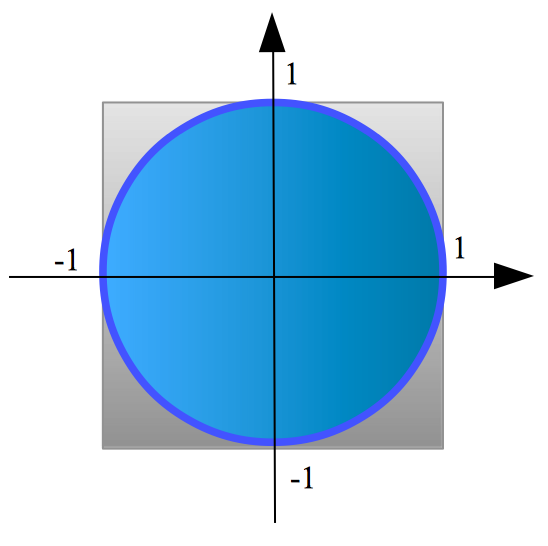
\includegraphics[scale=0.7]{aproximaPi.png}
\end{figure}

Por lo tanto consideramos la siguiente ecuaci\'on para el calculo de $\pi$:

\begin{equation}
H(x,y) = \begin{cases}  1 \text{ si } x^2 + y^2 \leq 1 \\ 
0 \text{ in other case }  \end{cases}
\end{equation}

\subsection{Desarrollo (secci\'on 1. Monte Carlo)}

\begin{itemize}
\item Pruebe el  c\'odigo en python proporcionado y ejecute pruebas para $N = 100, 1000, 10000, 100000, 1000000$, muestre cu\'ales son los valores que obtiene para $\pi$ en cada caso.

\begin{figure}[H]
\centering
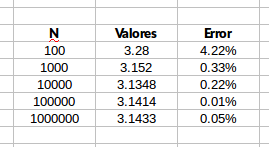
\includegraphics[scale=0.6]{tabla.png}
\label{fig:tabla Resultados}
\caption{se muestran los resultados de la experimentación}
\end{figure}

\item Implemente el m\'etodo de Monte Carlo para resolver integrales.
Utilice la siguiente formula:
\begin{equation}
\frac{b-a}{n} \sum_{i = 1}^{n}f(u_i(b-a) + a)
\end{equation}

donde $a$ y $b$ son los l\'imites inferior y superior de una integral, $u_i$ es un valor aleatorio generado entre $[0,1]$ y $f$ se refiere a la funci\'on a integrar.

Considere las siguientes integrales para probar su implementaci\'on:
\begin{equation}
f_1(x) = \int_{0}^{1} (1-x^2)^{3/2} \cdot dx
\end{equation}

\begin{equation}
f_2(x) = \int_{-1}^{1} e^{x+x^2} \cdot dx
\end{equation}

\begin{equation}
f_3(x) = \int_{0}^{2} (1+x^2)^2 \cdot dx
\end{equation}

\begin{equation}
f_4(x) = \int_{0}^{2\pi} \frac{1}{cos(x)+2} \cdot dx
\end{equation}

\begin{equation}
f_5(x) = \int_{0}^{2} log(x) \cdot dx
\end{equation}
\end{itemize}

Deber\'a desarrollar una simulaci\'on donde se muestre paso a paso la generaci\'on de n\'umeros aleatorios y su graficaci\'on en la funci\'on correspondiente. (Ver ejemplo en figura \ref{fig:interfaz} y consulte la p\'agina web https://www.scratchapixel.com/lessons/mathematics-physics-for-computer-graphics/monte-carlo-methods-in-practice/monte-carlo-integration). 

\begin{figure}[H]
\centering
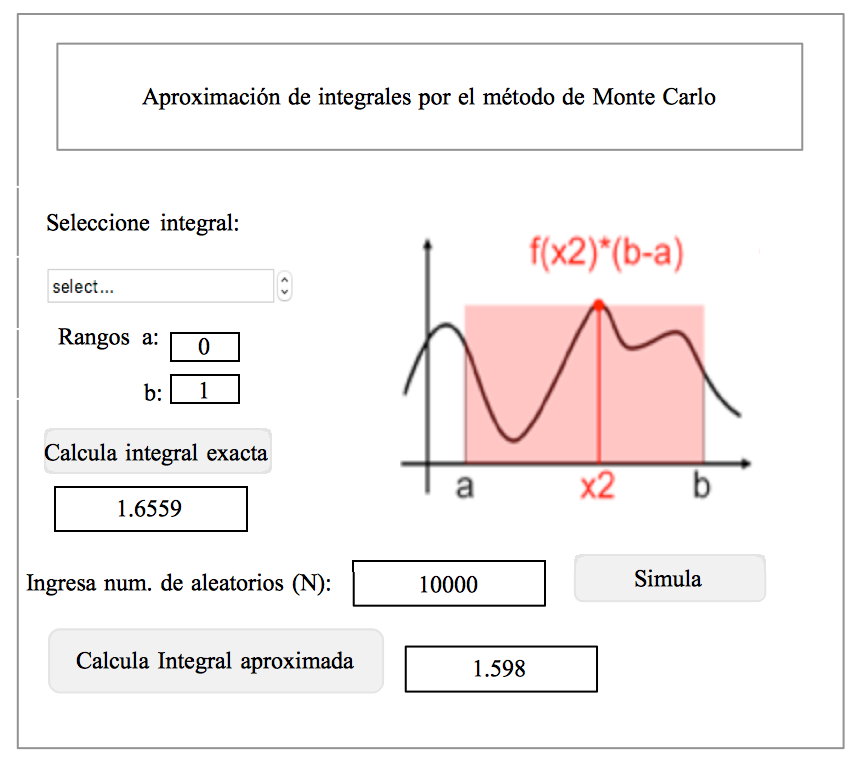
\includegraphics[scale=0.6]{Interfaz.png}
\label{fig:interfaz}
\caption{Ejemplo de interfaz gr\'afica para simular aproximaci\'on a integrales}
\end{figure}

\begin{figure}[H]
\centering
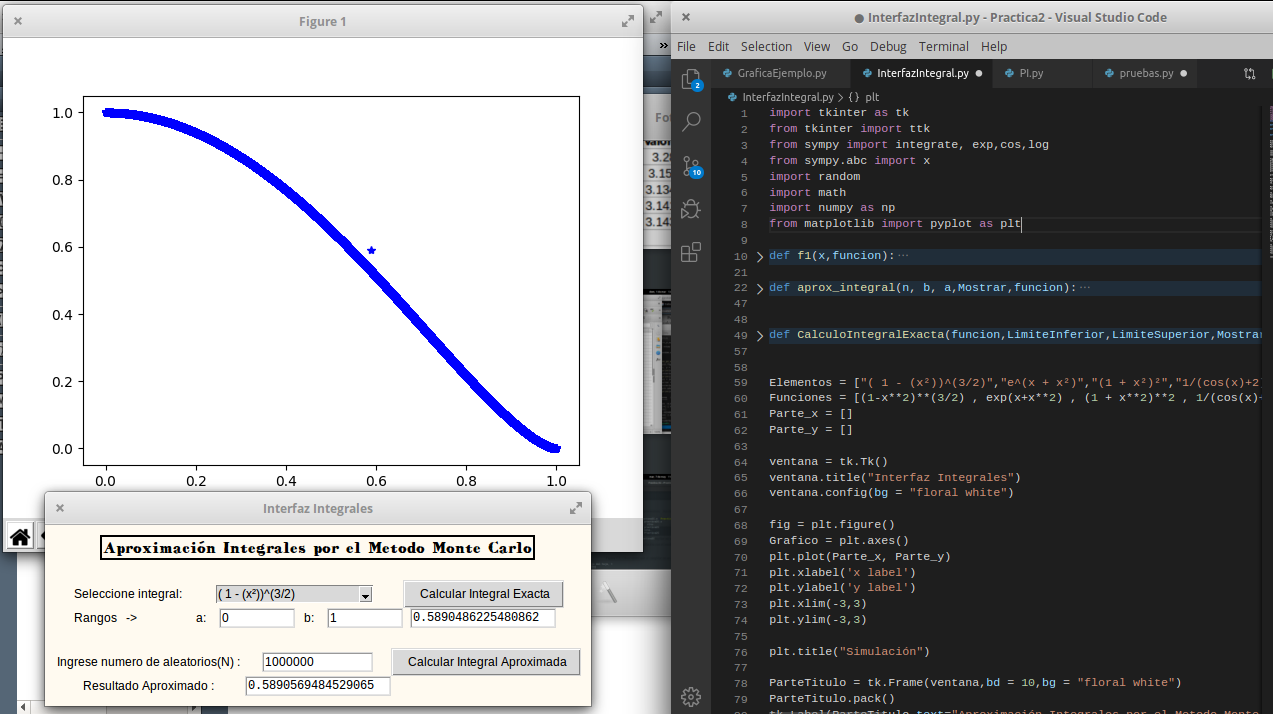
\includegraphics[scale=0.3]{interfazCreada.png}
\label{fig:Interfaz Hecha}
\caption{Interfaz gr\'afica para simular aproximaci\'on a integrales que se realiz\'o}
\end{figure}

\begin{lstlisting}
import tkinter as tk
from tkinter import ttk
from sympy import integrate, exp,cos,log
from sympy.abc import x
import random
import math
import numpy as np
from matplotlib import pyplot as plt

def f1(x,funcion):
    if funcion == 0:
        return ( 1 - x**2 )**( 3/2 )
    elif funcion == 1:
        return math.exp( x + x**2 )
    elif funcion == 2:
        return (1 + x**2 )**2
    elif funcion == 3:
        return 1/(math.cos(x) + 2)
    elif funcion == 4:
        return math.log(x)

def aprox_integral(n, b, a,Mostrar,funcion):
    Parte_x = []
    Parte_y = []
    sum  = 0
    for i in range(0, n):
        ui = random.uniform(0, 1)
        operacion = ui*(b-a) + a
        resultadoFuncion = f1(operacion,funcion)
        sum  = sum + resultadoFuncion
        Parte_x.append(operacion)
        Parte_y.append(resultadoFuncion)
    
    resultado = (b-a)/n * sum

    Mostrar.config(state="normal")
    Mostrar.delete(1.0, tk.END)
    Mostrar.insert(tk.END,resultado)
    Mostrar.config(state="disabled")    

    Parte_x.append(resultado)
    Parte_y.append(resultado)
    
    plt.cla()
    plt.plot(Parte_x,Parte_y,"b*")
    plt.show()


def CalculoIntegralExacta(funcion,LimiteInferior,LimiteSuperior,Mostrar):
    
    resultado = float(integrate(Funciones[funcion],
     (x,float(LimiteInferior),float(LimiteSuperior))))
 
    Mostrar.config(state="normal")
    Mostrar.delete(1.0, tk.END)
    Mostrar.insert(tk.END,resultado)
    Mostrar.config(state="disabled")


Elementos = ["( 1 - (x²))^(3/2)","e^(x + x²)","(1 + x²)²",
"1/(cos(x)+2)","log(x)"]
Funciones = [(1-x**2)**(3/2) , exp(x+x**2) , (1 + x**2)**2 ,
 1/(cos(x)+2) ,log(x)]
Parte_x = []
Parte_y = []

ventana = tk.Tk()
ventana.title("Interfaz Integrales")
ventana.config(bg = "floral white")

fig = plt.figure()
Grafico = plt.axes()
plt.plot(Parte_x, Parte_y)
plt.xlabel('x label')
plt.ylabel('y label')
plt.xlim(-3,3)
plt.ylim(-3,3)

plt.title("Simulación")

ParteTitulo = tk.Frame(ventana,bd = 10,bg = "floral white")
ParteTitulo.pack()
tk.Label(ParteTitulo,text="Aproximación Integrales por 
el Metodo Monte Carlo", borderwidth=2, relief="solid",
font=("HVD Bodedo",10),bg = "floral white").pack()

ParteEntradas = tk.Frame(ventana, bd = 10,bg = "floral white") 
ParteEntradas.pack()

tk.Label(ParteEntradas,text="Seleccione integral: ",
bg = "floral white").grid(row = 0,column = 0)
Opciones = ttk.Combobox(ParteEntradas,state = "readonly",
values = Elementos , width = 20)
Opciones.grid(row = 0,column = 1,columnspan= 4 )

tk.Label(ParteEntradas,text="Rangos   -> ",bg = "floral white").
grid(row = 1,column = 0,sticky = 'W')
LimiteInferior = tk.Entry(ParteEntradas,width = 10)

tk.Label(ParteEntradas,text="a: ",bg = "floral white",width = 4).
grid(row = 1,column = 1)
LimiteInferior.
grid(row = 1,column = 2)
tk.Label(ParteEntradas,text="b: ",bg = "floral white",width = 4).
grid(row = 1,column = 3)
LimiteSuperior = tk.Entry(ParteEntradas,width = 10)
LimiteSuperior.grid(row = 1,column = 4)

tk.Button(ParteEntradas, text=" Calcular Integral Exacta", height = 1,
 activebackground = "blue", activeforeground = "White",
 command = lambda: CalculoIntegralExacta(Opciones.current(),
 LimiteInferior.get(),LimiteSuperior.get(),
 
TextoIntegralExacta)).grid(row = 0,column = 5)
TextoIntegralExacta = tk.Text(ParteEntradas,width = 20,height = 1)
TextoIntegralExacta.insert(tk.END,"Solucion ")
TextoIntegralExacta.config(state = "disabled")
TextoIntegralExacta.grid(row = 1,column = 5)

ParteSimulacion = tk.Frame(ventana,bd = 10,bg = "floral white")
ParteSimulacion.pack()
tk.Label(ParteSimulacion,text="Ingrese numero de aleatorios(N) : ",
bg = "floral white").grid(row = 0,column = 0)
N = tk.Entry(ParteSimulacion,width = 15)
N.grid(row = 0,column = 1)
tk.Button(ParteSimulacion, text=" Calcular Integral Aproximada", 
height = 1, activebackground = "blue", activeforeground = "White",
command = lambda: aprox_integral(int(N.get()),float(LimiteSuperior.
get()),float(LimiteInferior.get()),
TextoIntegralAproximado,Opciones.current())).grid(row = 0,column = 2)

tk.Label(ParteSimulacion,text="Resultado Aproximado : ",
bg = "floral white").grid(row = 1,column = 0)
TextoIntegralAproximado = tk.Text(ParteSimulacion,width = 20,height = 1)
TextoIntegralAproximado.insert(tk.END,"Solucion ")
TextoIntegralAproximado.config(state="disabled")
TextoIntegralAproximado.grid(row=1,column=1)

ventana.mainloop()

\end{lstlisting}

\subsection{Desarrollo (secci\'on 2. Las Vegas )}

Para poner en pr\'actica el algoritmo las vegas se implementaran dos ejercicios:

\begin{enumerate}
	\item Algoritmo de Quick-sort. Modifique el algoritmo de Quick sort implementado en la pr\'actica 1. Por cada llamada recursiva seleccione al azar el pivote, compare si hay mejora respecto  a su versi\'on anterior para el caso promedio y reporte el tiempo de ejecuci\'on para los siguientes casos $n = 1000, 2000, 3000, \ldots, 10,000$ ($n$ es el n\'umero de elementos en un arreglo).
	\item El prolema de las 8 reinas. Se requiere generar una soluci\'on correcta al problema de las 8 reinas de acuerdo a las siguientes reglas.
\end{enumerate}

\begin{lstlisting}
CODIGO QUICK-SORT

import random 
import timeit

def quicksort(arr, start, stop): 
    if(start < stop): 
          
        # pivotindex is the index where 
        # the pivot lies in the array 
        pivotindex = partitionrand(arr, start, stop) 
          
        # At this stage the array is partially sorted  
        # around the pivot. separately sorting the  
        # left half of the array and the right half of the array. 
        quicksort(arr , start , pivotindex) 
        quicksort(arr, pivotindex + 1, stop) 
  
# This function generates random pivot, swaps the first 
# element with the pivot and calls the partition function. 
def partitionrand(arr , start, stop): 
    randpivot = random.randrange(start, stop) 
    arr[start], arr[randpivot] = arr[randpivot], arr[start] 
    return partition(arr, start, stop) 
  

def partition(arr,start,stop): 
    pivot = start # pivot 
    i = start - 1
    j = stop + 1
    while True: 
        while True: 
            i = i + 1
            if arr[i] >= arr[pivot]: 
                break
        while True: 
            j = j - 1
            if arr[j] <= arr[pivot]: 
                break
        if i >= j: 
            return j 
        arr[i] , arr[j] = arr[j] , arr[i] 

best_case = []
worst_case = []
rand_case = []
for i in range(10):
    f = open('best_case/b_' + str(i+1) + "000", 'r')
    x = f.read().split()
    best_case.append(x)
    f.close()

for i in range(10):
    f = open('rand_case/rand_' + str(i+1) + "000", 'r')
    x = f.read().split()
    rand_case.append(x)
    f.close()

for i in range(10):
    f = open('worst_case/w_' + str(i+1) + "000", 'r')
    x = f.read().split()
    worst_case.append(x)
    f.close()


f= open("data","w+")
for i in range(10):
    start= 0
    end = 0
    start = timeit.timeit()
    quicksort(best_case[i],0, len(best_case[i])-1 )
    end = timeit.timeit()
    f.write(str(end) +  ", ")
    print(end - start)

f.write("\n")

for i in range(10):
    start = timeit.timeit()
    quicksort(worst_case[i],0, len(worst_case[i])-1 )
    end = timeit.timeit()
    f.write(str(end) +  ", ")
    print(end - start)
f.write("\n")

for i in range(10):
    start = timeit.timeit()
    quicksort(rand_case[i],0, len(rand_case[i])-1 )
    end = timeit.timeit()
    f.write(str(end) +  ", ")
    print(end - start)


# array = [10, 7, 8, 9, 1, 5] 
# start = timeit.timeit()
# quicksort(array, 0, len(array) - 1)
# end = timeit.timeit()

# print(array) 

print(end - start)



f.close()

print(end - start)
\end{lstlisting}

\begin{lstlisting}
TIEMPOS QUICK-SORT
-Mejor Caso
	N		Tiempo
	100:	0.005853399999978137
	200: 	0.005635400000755908
	300:	0.005375199998525204
	400:	0.007245799999509472
	500:	0.005091899998660665
	600:	0.005041200000050594
	700:	0.0055608000002393965
	800:	0.005019500000344124
	900:	0.005019799998990493
	1000:	0.005130800000188174

-Peor Caso
	N		Tiempo
	100:	0.005725000000893488
	200:	0.005246299999271287
	300:	0.005106699998577824
	400:	0.005185100000744569
	500:	0.00503509999907692
	600:	0.005808799998703762
	700:	0.005068500000561471
	800:	0.005053700000644312
	900: 	0.005033600000388105
	1000:	0.005040399999415968
	
-Caso Random
	N		Tiempo
	100:	0.005251299999144976
	200:	0.005269900000712369
	300: 	0.005247099999905913 
	400:	0.005210300001635915
	500:	0.0050253999997948995
	600:	0.005389100000684266
	700:	0.005251699998552795
	800:	0.00606819999848085
	900: 	0.005101500000819215
	10000:	0.0056162000000767875,  
\end{lstlisting}

El problema de las 8 reinas consiste en colocar las piezas en un tablero de ajedrez sin que se amenacen entre s\'i. En el juego de ajedrez la reina amenaza a aquellas piezas que se encuentren en su misma fila, columna o diagonal. 

Para resolver este problema emplearemos un esquema de algoritmo Las vegas. Se supondr\'a que hay un cierto n\'umero de piezas colocadas en forma correcta (sin atacarse) y se generar\'a el resto de las piezas al azar.
Considera las siguientes configuraciones predefinidas e implemente un algoritmo que genere las otras reinas de manera aleatoria.

\begin{lstlisting}
CODIGO QUEEN

class NQueens:
    """Generate all valid solutions for the n queens puzzle"""
    def __init__(self, size):
        # Store the puzzle (problem) size and the number of valid solutions
        self.size = size
        self.solutions = 0
        self.solve()

    def solve(self):
        positions = [-1] * self.size
        self.put_queen(positions, 0)
        print("Found", self.solutions, "solutions.")

    def put_queen(self, positions, target_row):
        # Base (stop) case - all N rows are occupied
        if target_row == self.size:
            self.show_full_board(positions)
            self.solutions += 1
        else:
            # For all N columns positions try to place a queen
            for column in range(self.size):
                # Reject all invalid positions
                if self.check_place(positions, target_row, column):
                    positions[target_row] = column
                    self.put_queen(positions, target_row + 1)

    def check_place(self, positions, ocuppied_rows, column):
        for i in range(ocuppied_rows):
            if positions[i] == column or \
                positions[i] - i == column - ocuppied_rows or \
                positions[i] + i == column + ocuppied_rows:

                return False
        return True

    def show_full_board(self, positions):
        for row in range(self.size):
            line = ""
            for column in range(self.size):
                if positions[row] == column:
                    line += "Q "
                else:
                    line += ". "
            print(line)
        print("\n")

NQueens(8)
\end{lstlisting}


\end{document}
